\documentclass[letterpaper,10pt,twocolumn,titlepage]{article}

\usepackage{graphicx}                                        
\usepackage{amssymb}                                         
\usepackage{amsmath}                                         
\usepackage{amsthm}                                          

\usepackage{alltt}                                           
\usepackage{float}
\usepackage{color}
\usepackage{url}

\usepackage{balance}
\usepackage[TABBOTCAP, tight]{subfigure}
\usepackage{enumitem}
\usepackage{pstricks, pst-node}

\usepackage{fancyhdr}
\pagestyle{fancy}
\usepackage{geometry}
\geometry{textheight=8.5in, textwidth=6in}

%random comment

\newcommand{\cred}[1]{{\color{red}#1}}
\newcommand{\cblue}[1]{{\color{blue}#1}}

\usepackage{hyperref}
\usepackage{geometry}

\def\name{Jonah Brooks}

%% The following metadata will show up in the PDF properties
\hypersetup{
  colorlinks = true,
  urlcolor = black,
  pdfauthor = {\name},
  pdfkeywords = {cs311 ``operating systems'' thread pthread prime},
  pdftitle = {CS 311 Project 3: Finding Prime Numbers},
  pdfsubject = {CS 311 Project 3},
  pdfpagemode = UseNone
}

\begin{document}

\fancyhead[R]{Jonah Brooks \linebreak CS311 HW3 \linebreak 02-23-2012}


\section{Finding Prime Numbers}
In this project, I wrote a program (h3.cpp) to find all prime numbers less than 2\textsuperscript{32}
using the Sieve of Eratosthenes. The graph comparing runtime to the number of threads used is on the final
page of this document.
 
\section{Design Decisions}
My original intent was to use a mixture of serial and parallel code, calculating all primes under 2\textsuperscript{16}
in serial, then checking divisibility of key numbers from there. I chose this approach so that there would be no conflicts
between threads. I optimized this as much as a could, but eventually gave up due to it using too much brute force.

My second attempt was a combination between my first attempt and a very modified version of the Sieve of Eratosthenes,
hoping that I could take a more elegant approach while still entirely avoiding thread collisions. However, this method
was also extremely inefficient. I toyed with the idea of running this method in some of the threads while running a pure
Sieve of Eratosthenes in a few others.

Ultimately, however, I chose a pure Sieve of Eratosthenese do the relatively simple nature of the algorithm, and opportunity
for optimization. I was able to get my running time down to a little under a minute, which is much, much better than my first two attempts,
but still well short of what I feel would be possible even with this algorithm. I optimized it as much as I could, but I was still
running into many thread collisions and required frequent use of mutexes. If I remove the use of mutexes when writing to the bitmap
I can halve the run time, but then I get many false positives. Using multiple bitmaps may well speed things up, but would require
far too much memory.

On the topic of mutexes, I chose to use one to protect the variable that stores the largest processed prime, as well as multiple
mutexes to lock sections of the bitmap. Originally I was planing to have one mutex for every byte in my bitmap, but the memory
constraints made this impossible. I tried implementing as many mutexes as I could, figuring the more the better, but after some testing
I discovered that there is some sweet spot for how many mutexes I wanted to use. Using only one (ie, locking the entire bitmap for every
entry) was extremely slow, as it created near serialization of my code. On the other hand, running as many mutexes as I can fit in memory
ran just as slowly. I am not sure why... perhaps the memory access time was taking too long. Either way, I found that it was optimal
to put 1024 bytes into each mutex.

Lastly, I chose to split my code into many different functions. This may not be the optimal approach for run time, especially since I
chose to rely on functions for converting between a number and its location in the bitmap. However, this made my code much easier to 
write and understand, so I am happy with this decision.

\vfill\break

\section{Commit Log}

\begin{tabular}{ | p{3cm} | p{5.5cm} | }
	\hline
	Commit Time & Commit Message \\ \hline
	\input{git_log_table}
\end{tabular}


\newpage
\newpage
\clearpage
\newpage
\clearpage
\clearpage
\newpage
\fancyhead{}

\begin{figure}[t!]
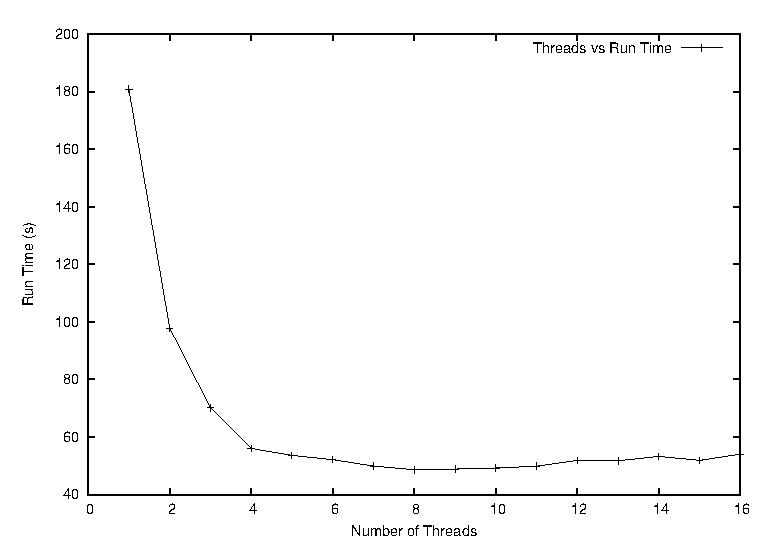
\includegraphics{time_graph.eps}
\end{figure}

\end{document}
















